\chapter{Generating Code for Graph Programs on a Manycore Architecture}\label{gen:sec:graphitbackend}
\markboth{Generating Code for Manycore Graph Programs}{Generating Code for Manycore Graph Programs}
%\newcommand{\nonblockedMethodFigure}{
\begin{figure}[h]
    \centering
    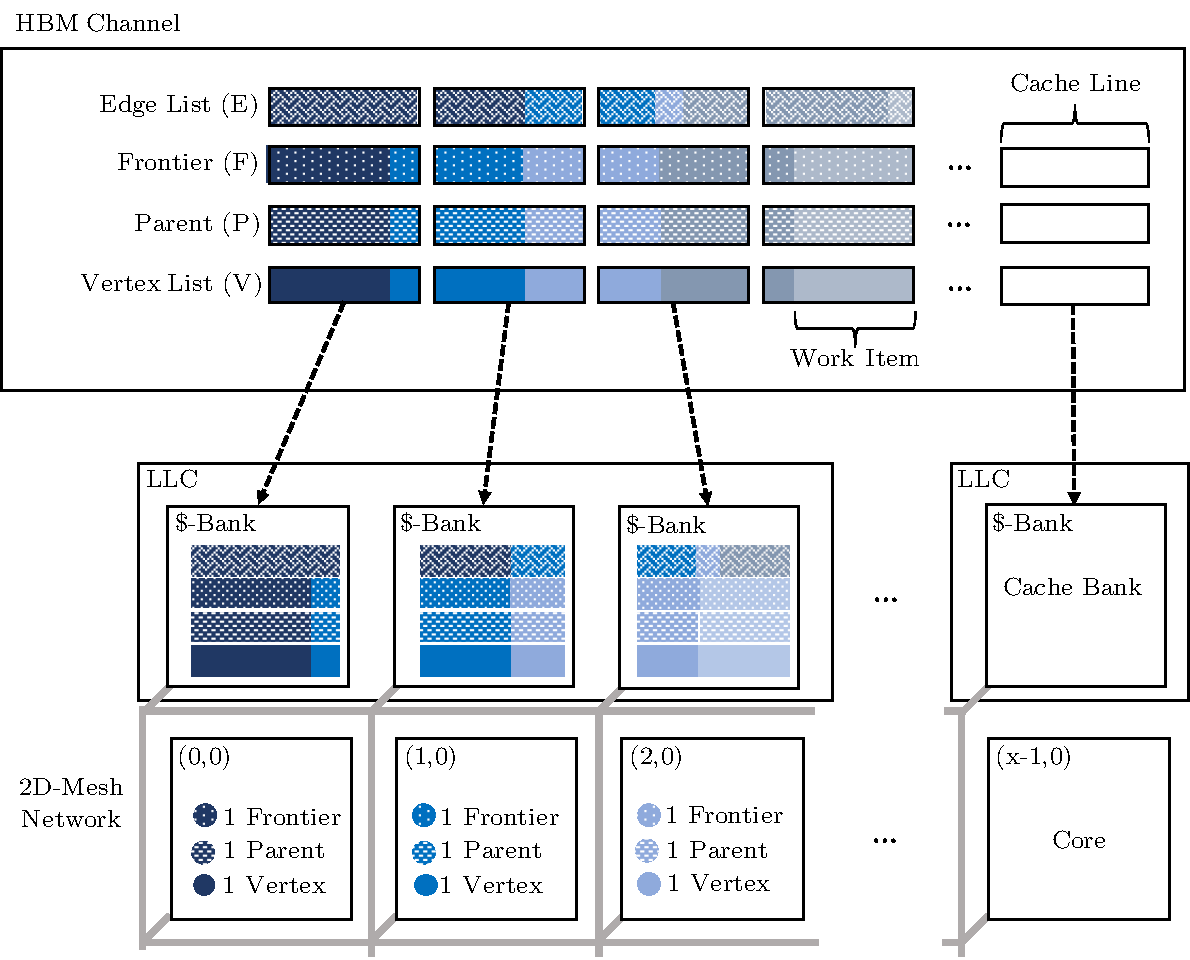
\includegraphics[scale=0.7]{graphit-figures/non-blocked.pdf}
    \caption{Data layout of BFS on the manycore. Data resides in HBM main memory and is cached in LLC. Each core is assigned work items sized without alignment consideration. Cores request single words of data on demand when needed. }
    \label{pap:generals:sec:method:sub:blocked:fig:non-blocked}
\end{figure}
}

\newcommand{\blockedMethodFigure}{
\begin{figure}[t]
    \centering
    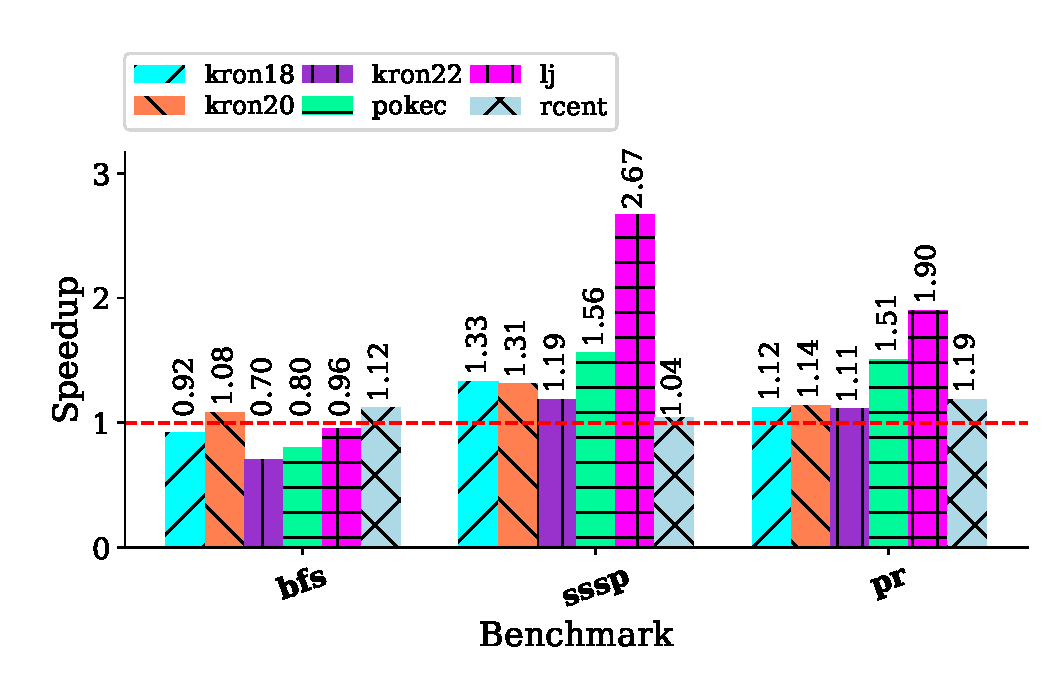
\includegraphics[scale=0.7]{graphit-figures/blocked.pdf}
    \caption{Data layout of BFS with blocked accesses. Cores are assigned cache aligned work items. Cores prefetch entire cache line-sized blocks of data to hide request latency.}
    \label{pap:generals:sec:method:sub:blocked:fig:blocked}
\end{figure}
}

\newcommand{\combinedBlockingFigure}{
\begin{figure*}[t!]
    \centering
    \subfloat[Non-Blocked Accesses]{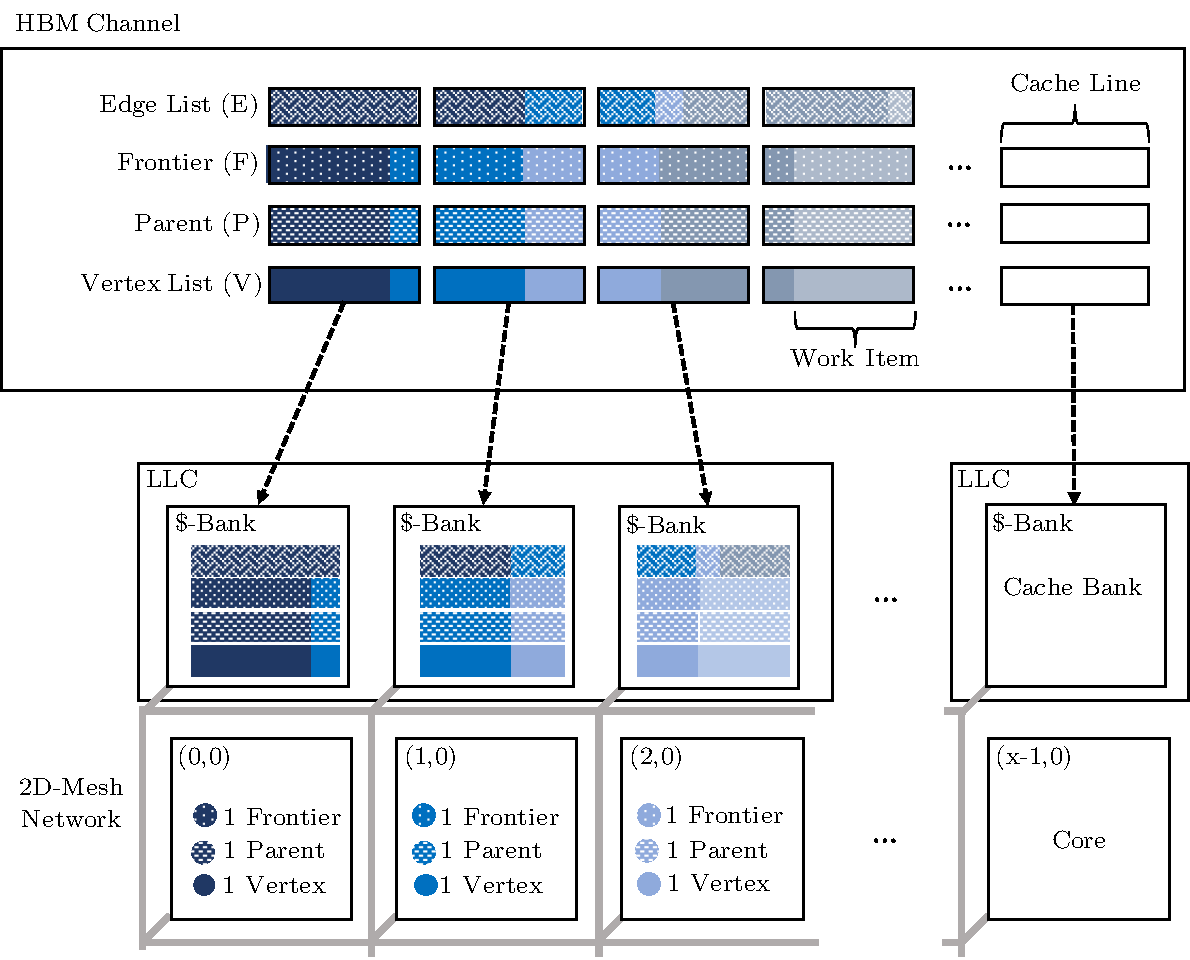
\includegraphics[scale=0.7]{graphit-figures/non-blocked.pdf}}
    \qquad
    \subfloat[Blocked Accesses]{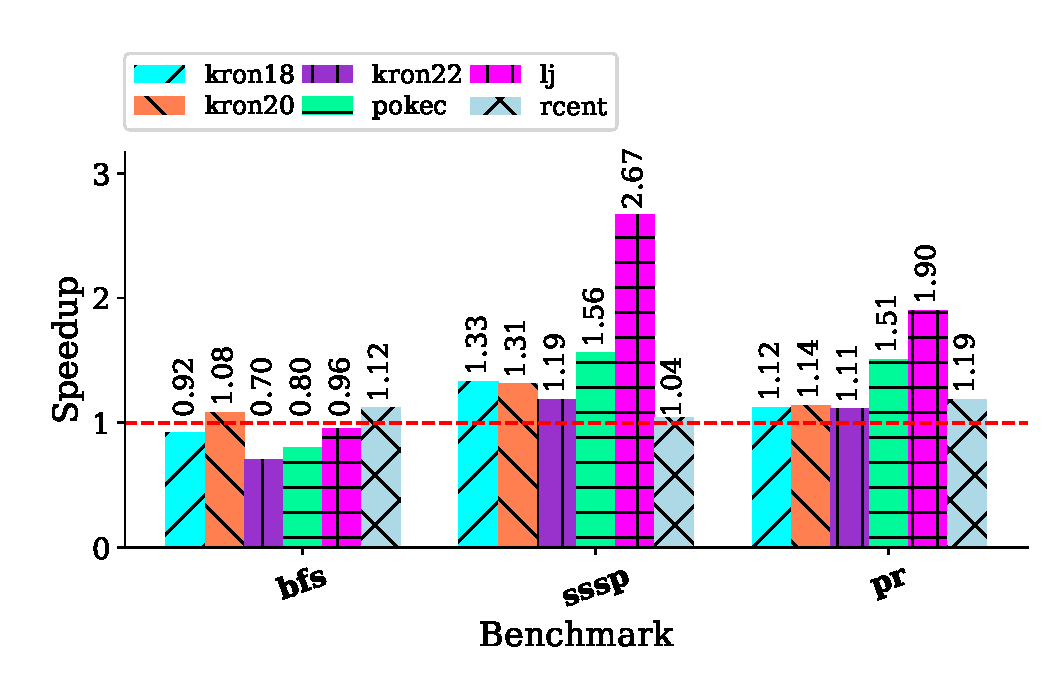
\includegraphics[scale=0.7]{graphit-figures/blocked.pdf}}
    \caption{Data layout of BFS on the manycore. Data resides in HBM main memory and is cached in LLC. In the baseline implementation, each cores are assigned work items sized without alignment consideration and request single words of data on demand when needed. With the blocked access optimization, cores are assigned cache aligned work items and prefetch entire line-sized blocks of data to hide request latency.}
    \label{pap:generals:sec:method:sub:blocked:fig:blocking}
\end{figure*}
}

\newcommand{\edgeAwareMethodFigure}{
\begin{figure}
    \centering
    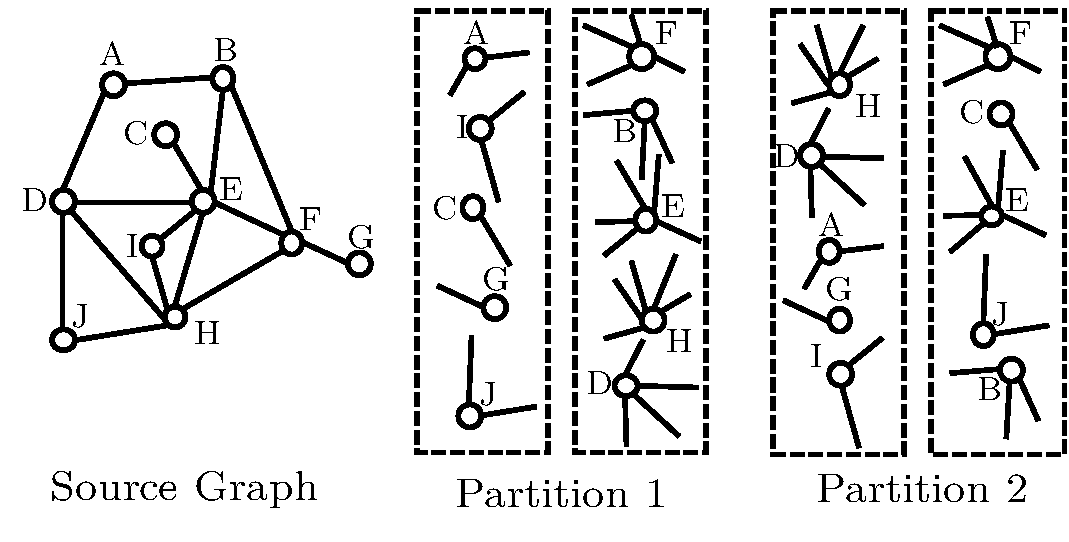
\includegraphics[scale=0.6]{graphit-figures/edge-aware.pdf}
    \caption{Depiction of vertex-based and edge-aware vertex-based partitioning. Partition 1 shows an example vertex-based partitioning between two cores, and Partition 2 shows an example edge-aware partitioning that provides a better workload balance between the two cores.}
    \label{fig:edgeaware}
\end{figure}
}
\newcommand{\edgeAwareMethodAlgorithm}{
\begin{figure}
\centering
\begin{algorithmic}[1]
\Function{Recursive Range}{$start, end$}
\If {$index[end] - index[start] < grain size$}
    \State $core.start \gets start$
    \State $core.end \gets end$
\Else 
    \State $recursive range (start, end/2)$
    \State $recursive range (end/2, start)$
\EndIf
\EndFunction
\end{algorithmic}
\caption{Pseudocode for the recursive call portion of the edge-aware vertex partitioning scheme.}
    \label{alg:edge-aware}
\end{figure}
}
\newcommand{\pushVPullMethodFigure}{
\begin{figure}
    \centering
    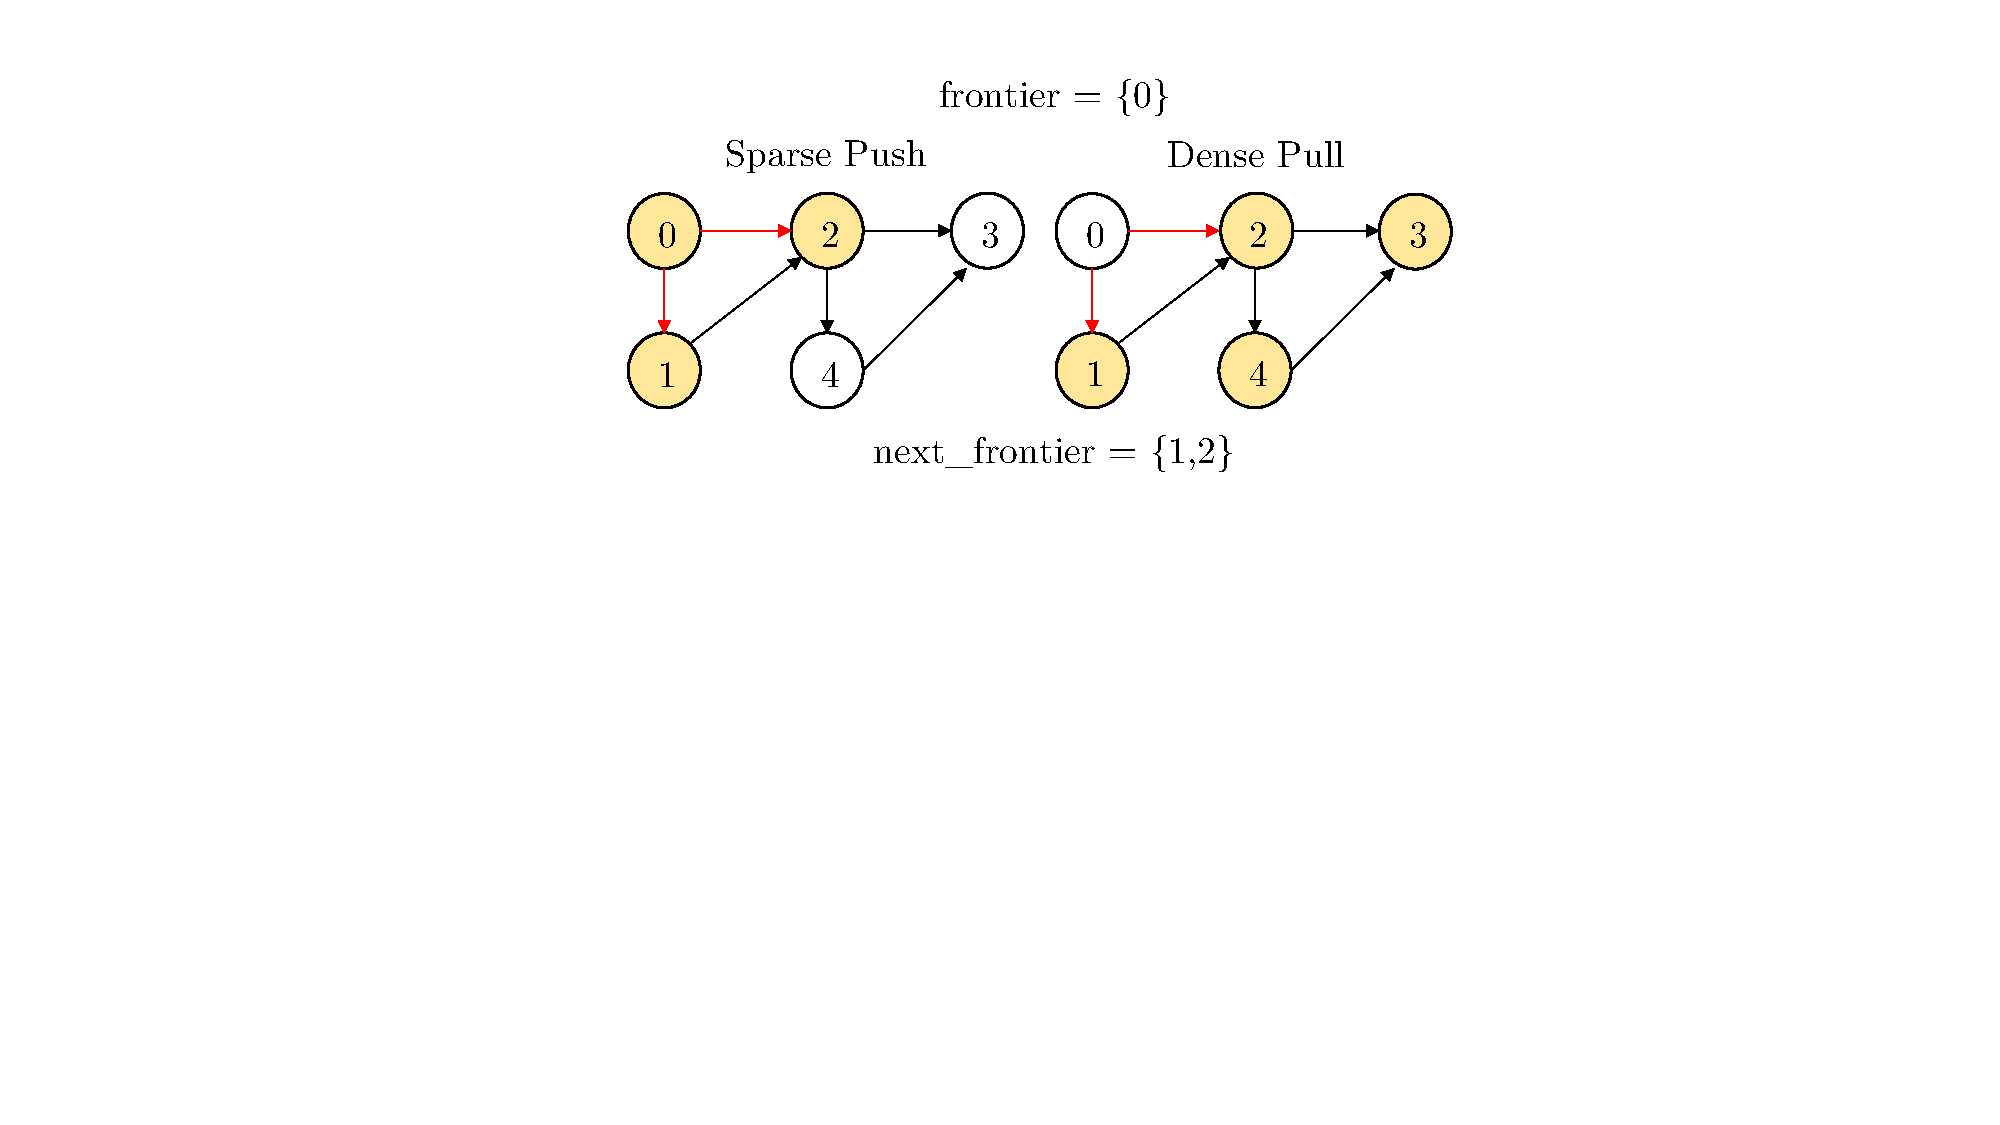
\includegraphics[scale=0.7]{graphit-figures/push_v_pull_fig.pdf}
    \caption{Representation of one iteration of BFS in both the \textsc{Push} and \textsc{Pull} directions. Nodes highlighted in yellow are visited during the iteration. Edges in red are edges that are traversed during execution.}
    \label{fig:pushpull}
\end{figure}
}

\introOverviewFigure

%\todo{intro paragraph to discuss the problem with graph processing again?/contextualize after background and related work?}
To harness the benefits of manycore architectures and reduce programming complexity, we propose a code generation backend for GraphIt, a flexible domain-specific language (DSL) for graph computations~\cite{zhang2018graphit}. 
We implement our backend as a \graphvm using \ugc.
This backend generates code targetting the representative manycore architecture described in \ref{gen:sec:background}.
We use this new backend to implement and explore the performance of the optimizations discussed in Chapter~\ref{gen:sec:optimizations}.
%Our evaluation shows that our GraphIt backend achieves a maximum of 467.1 million traversed edges per second (MTEPS) and on average achieves 252.7 MTEPS across all input graphs and benchmarks studied. 
%We find that our optimizations achieve a maximum speedup of 2.1$\times$ and an average speedup of 1.16$\times$ over naive manycore implementations.
An overview of our approach is shown in Figure~\ref{pap:generals:sec:intro:fig:overview}.

\section{Manycore Code Generation}\label{sec:method:sub:baseline}

Reasoning about these performance optimizations and manycore-specific considerations is a challenging task.
To address this, we developed a code generation backend targeting a manycore architecture.
This code generator alleviates the need for the programmer to have extensive knowledge of the underlying architecture.
%To alleviate the need for the programmer to have knowledge of the underlying manycore architecture, we develop a code generation backend to GraphIt targeting a manycore architecture.

We add support for our backend and the manycore specific optimizations discussed in Chapter~\ref{gen:sec:optimizations} by implementing a \hb scheduling language using the abstract language provided by \GG.
%First, we added the option \lstinline[language=graphit]{generateManycoreCode()} which signals to the GraphIt compiler it should generate code for the manycore architecture described in Section~\ref{pap:generals:sec:architecture}.
This scheduling language signals to the \graphit compiler that it should generate code for the \hb~manycore architecture.
We also add support for each of the optimizations described in Chapter~\ref{gen:sec:optimizations} including our blocked access method and alignment-based partitioning scheme.

In order to generate code that runs on the manycore, we must generate code for both the host CPU and the manycore device.
%An early consideration when designing the backend was how to split the code between host and device. 
We chose to have the host code handle setup and coordination and to have the device code handle the core graph work.
This is a natural split as it allows the manycore to handle the parallel portions of execution and lets the CPU handle the serial portions of work that require an operating system.

\subsection{Host Code} 

The host code that we generate handles most of the setup and coordination of the graph program. 
We leverage a set of runtime libraries that we wrote to simplify and generalize the code generation. 
These runtime libraries provide wrappers over our host driver API and handle loading of program data into manycore memory, initializing the manycore and initiating kernel execution on the manycore. 
These runtime libraries provide a level of abstraction which allows for seamless portability of our backend. 
In order to target a different manycore architecture, we would only need to modify these wrapper functions and would not need to modify our code generator.
\newline
\lstset{language=C++,
captionpos=b,
xleftmargin=.05\textwidth,
frame=single,
numbers=left,
framerule=0pt,
aboveskip=1pt,
belowskip=1pt,
framesep=1pt,
basicstyle=\footnotesize\ttfamily,
keywordstyle={[1]\color{darkcandyapplered}},
keywordstyle={[2]\color{blue}},
keywordstyle={[3]\color{black}\bfseries},
keywordstyle={[4]\color{darkcandyapplered}\bfseries},
emphstyle=\slshape,
commentstyle=\color{darkgray},
stringstyle=\color{darkgreen}
}
\begin{lstlisting}[language=C++, breaklines=true, 
                   caption=Generated manycore host code for the Breadth-First Search (BFS) program shown in Listing~\ref{pap:generals2020:sec:background:lst:graphit}.,
                   label=pap:generals:sec:method:lst:host]
Graph edges = loadEdgesFromFile(file_path) ;
Vector<int> frontier = new Vector<int>(
        edges.num_nodes(), 0);
Device::Ptr device = Device::GetInstance();
addVertexOnDevice(frontier, root );
while (getVertexSetSizeDevice(frontier) != 0){
      device->enqueueJob("bfs_pull_call",
          {edges.getInIndicesAddr() , 
           edges.getInNeighborsAddr(), 
           frontier.getAddr()}); 
      device->runJobs();
}
\end{lstlisting}
Listing~\ref{pap:generals:sec:method:lst:host} shows a subset of the host code generated for the BFS program shown in Listing~\ref{pap:generals2020:sec:background:lst:graphit} and highlights some of our host side runtime libraries for coordinating placement of data and scheduling of work.

The function \lstinline[language=C++, basicstyle=\small\ttfamily]{loadEdgesFromFile} on line~1 loads a graph from an edgelist, formats the graph into the CSR storage format, and loads it into HBM. 
We also provide functions such as \lstinline[language=C++, basicstyle=\small\ttfamily]{addVertexOnDevice} shown on line~4, which handles the insertion of values into vectors that are stored in HBM. 
Finally, on lines 7 and 11 we have functions for scheduling kernel execution on the manycore: \lstinline[language=C++, basicstyle=\small\ttfamily]{enqueueJob()} and \lstinline[language=C++, basicstyle=\small\ttfamily]{runJobs()}.
The enqueue job function takes the name of a kernel along with a list of parameters for that kernel and schedules it for execution.
Lines~8-10 show the functions we provide to find the address of data structures stored in HBM. 
For vector types, we provide the \lstinline[language=C++, basicstyle=\small\ttfamily]{getAddr()} method.
For graphs, we provide \lstinline[language=C++, basicstyle=\small\ttfamily]{getInIndicesAddr()} and \lstinline[language=C++, basicstyle=\small\ttfamily]{getInNeighborsAddr()} to get the addresses of the index and neighbor arrays respectively.
The \lstinline{runJobs()} function tells the manycore to execute all jobs that have been scheduled through calls to \lstinline[language=C++, basicstyle=\small\ttfamily]{enqueueJob()}.

\subsection{Device Code}

All \lstinline[language=graphit]{vertexset} and  \lstinline[language=graphit]{edgeset} operators are generated as device code. Most importantly, this includes apply and filter operations along with the edgeset apply modified operation. 
By default, all of these operators are generated as parallel kernels meant to be executed across the entire manycore. 
To distribute work among cores, we implement a \lstinline[language=C++, basicstyle=\small\ttfamily]{local_range(V, start, end)} library function that takes as input the total number of vertices, a pointer to a start value, and a pointer to an end value.
The function evenly splits the vertices across the cores and sets the start and end values as a contiguous subset of vertices for each core to work on. 
Our backend replaces the call to \lstinline[language=C++, basicstyle=\small\ttfamily]{local_range} with \lstinline[language=C++, basicstyle=\small\ttfamily]{edge_aware_local_range} to do the recursive edge-aware work assignment described in Chapter~\ref{sec:method:sub:edge-aware-partitioning}.
\newline
\begin{lstlisting}[language=C++, breaklines=true, 
                   caption=Generated manycore device code for the Breadth-First Search (BFS) program shown in Listing~\ref{pap:generals2020:sec:background:lst:graphit}.,
                   label=pap:generals:sec:method:lst:device]
template <typename TO_FUNC, typename APPLY_FUNC> int bfs_pull(int *in_indices , int *in_neighbors, int *from_vertexset, TO_FUNC to_func, APPLY_FUNC apply_func) { 
    int start, end;
    local_range(V, &start, &end);
    for ( int d = start; d < end; d++) {
        if (to_func(d)){ 
            for(int s = in_indices[d]; s < in_indices[d+1]; s++) {
                if(from_vertexset[s] == 1) {
                    if(apply_func( in_neighbors[s], d )){ 
                        next[d] = 1; 
                    }
                }
            } //end of loop on in neighbors
        } //end of to filtering
    } //end of outer for loop
    barrier.sync();
    return 0;
}
\end{lstlisting}

Listing~\ref{pap:generals:sec:method:lst:device} shows the main kernel code generated for the inner loop of BFS. 
In this code, we can see the use of the \lstinline[language=C++, basicstyle=\small\ttfamily]{local_range} function on line~3 and the use of a barrier before each core exits the kernel on line~15. 
Lines~4-14 iterate through all of the vertices in the graph, traverse edges that have not yet been visited, and build the next frontier.
The parallelism is achieved by each core executing their own contiguous range of vertices obtained from \lstinline[language=C++, basicstyle=\small\ttfamily]{local_range} at the same time. Once a core is finished with its computation, it waits at the barrier for all other cores to finish before returning the results of the iteration. 

\paragraph{Atomics}\mbox{}\\
While atomics can mostly be avoided when traversing in the \pull direction, they are still necessary in some cases and are always necessary during \push traversal.
We leverage lock data structures to implement the necessary atomic operations used in our device code.
We initialize one lock per cache line in the LLCs.
Our profiling showed that this number of locks was sufficient to reduce contention in lock acquisition.
Locks are assigned using a simple hash function on the address of the element for which an atomic operation has been called.

\section{Chapter Summary}
In this chapter we introduced our \hb code generation backend.
Our code generator allows a user to easily reason about a variety of graph processing and manycore-specific optimizations.
We described how we generate code for both the host processor and manycore device. 
We choose to have the host processor handle coordination and initialization while the device computes the graph traversals and updates.